\documentclass{beamer}
\usepackage{minted}
\usepackage{tikz}
\usepackage{xcolor}
\usetikzlibrary{positioning} 
\usetikzlibrary{arrows.meta}

\title{edX Load Tests}
\subtitle{Introduction And Current Status}
\author{Troy Sankey}
\date{\today}

\begin{document}


\begin{frame}
\titlepage
\end{frame}

\begin{frame}
\frametitle{Introduction}
\setbeamercovered{invisible}
\begin{itemize}
\item Tests live in the edx/edx-load-tests repo.\pause
\item Uses the Locust load testing tool.
\end{itemize}
\end{frame}


\begin{frame}
\frametitle{Why Load Test?}
\setbeamercovered{invisible}
\begin{itemize}
% * One reason is to measure performance improvements to check your
%   assumptions.
\item Performance-related improvements.\pause
% * But we also don't want to let regressions fall through the cracks.
\item Performance-sensitive code changes.
\item Major version changes of dependencies.
% * In the past, people have load tested:
%   - Docker Devstack
%   - Upgrading ES
%   - New course home page
\end{itemize}
\end{frame}


\begin{frame}
\frametitle{Overview Of Writing Tests}
\setbeamercovered{invisible}
\begin{enumerate}
\item Identify endpoints.\pause
\item Write tasks for each endpoint.\pause
\item Write startup (\texttt{on\_start()}) function.\pause
\item Write instructions for seeding test data.
\end{enumerate}
\end{frame}


% Macro for highlighting blocks of code without affecting text positioning.
\newcommand{\highlight}[1]{%
  \begingroup
  \setlength{\fboxsep}{0pt}%  
  \colorbox{yellow}{\strut#1}%
  \endgroup
}
\setminted{fontsize=\small,escapeinside=||,linenos}


% * Locust tests are basically randomly selected python functions (tasks)
%   repeatedly executed.
% * Tasks are leaf nodes in a tree of TaskSet nodes.
% * TaskSets represent different kinds of activities a user engages in.  For
%   example in our LMS load test the forums-related tasks are grouped inside
%   the ForumsTasks TaskSet.
\begin{frame}[fragile]
\frametitle{\texttt{locustfile.py}}
\begin{minted}{python}
class ChatTasks(TaskSet)
    @task(3)
    def send_message():
        print("sending a message.")
    @task(8)
    def get_emoji():
        print("getting list of emoji.")

class ServiceTasks(TaskSet):
    tasks = {
        ChatTasks: 1,
        SearchTasks: 2,
    }

class ServiceUser(HttpLocust):
    task_set = ServiceTasks
    min_wait = 1000
    max_wait = 5000
\end{minted}
\end{frame}


% * In this example, ServiceTasks is the root TaskSet representing the entire
%   service.
% * Locusts select which task to execute using the probability distributions
%   defined by the tasks class variable.
% * Each task under ServiceTasks happens to be references to other TaskSets.
\begin{frame}[fragile]
\frametitle{\texttt{locustfile.py}}
\begin{minted}{python}
class ChatTasks(TaskSet)
    @task(3)
    def send_message():
        print("sending a message.")
    @task(8)
    def get_emoji():
        print("getting list of emoji.")

class |\highlight{ServiceTasks}|(TaskSet):
    tasks = {
        ChatTasks: 1,
        SearchTasks: 2,
    }

class ServiceUser(HttpLocust):
    task_set = |\highlight{ServiceTasks}|
    min_wait = 1000
    max_wait = 5000
\end{minted}
\end{frame}


% * ChatTasks represents an activity for users on the the service
% * The tasks in this example correspond to some possible AJAX calls from the
%   client browser.
\begin{frame}[fragile]
\frametitle{\texttt{locustfile.py}}
\begin{minted}{python}
class |\highlight{ChatTasks}|(TaskSet)
    @task(3)
    def send_message():
        print("sending a message.")
    @task(8)
    def get_emoji():
        print("getting list of emoji.")

class ServiceTasks(TaskSet):
    tasks = {
        |\highlight{ChatTasks}|: 1,
        SearchTasks: 2,
    }

class ServiceUser(HttpLocust):
    task_set = ServiceTasks
    min_wait = 1000
    max_wait = 5000
\end{minted}
\end{frame}


\begin{frame}
\frametitle{User Experience}
\setbeamercovered{invisible}
\begin{itemize}
\item No browser, no javascript, no good measure of user experience.
\item Focus on the system response, not the users.
% * Now that you've seen an example locustfile, you may have noticed the tasks
%   are relatively low-level.
% * If you want, during a load test you could login from a browser to measure
%   user experience.
\end{itemize}
\end{frame}


\begin{frame}
\frametitle{Settings}
\begin{itemize}
\item Each load test is configurable via a YAML file.\pause
% * This wasn't always the case, do not revert back to reading environment
%   variables!
% * Settings module improves test reproducability and clarity.
\item Use \texttt{helpers.settings}.\pause
\item The Jenkins job (run-simple-loadtest) will use settings specified by a
      job parameter.
\end{itemize}
\end{frame}


\tikzstyle{title} = [text centered, text width=12em]
\tikzstyle{base} = [rectangle, draw=black, text centered, text width=12em]
\tikzstyle{mstep} = [base]
\tikzstyle{to} = [->,>={Latex[width=2mm,length=2mm]}]
\tikzstyle{to-emph} = [to,ultra thick]
\tikzstyle{to-deemph} = [to,opacity=0.3]

\begin{frame}
\frametitle{Overview Of Running Load Tests}
\setbeamercovered{invisible}
\begin{center}
\begin{tikzpicture}
\node[title] (rightColumn) {Target};
\node[mstep, below=1em of rightColumn] (loadtest) {Loadtest Environment};\pause
\node[title, left=of rightColumn] (leftColumn) {Source};
\node[mstep, left=of loadtest] (runLoadtest) {run-simple-loadtest (jenkins)};
\uncover<-6>{\draw[to] (runLoadtest) -- (loadtest);}\pause
\node[mstep, below=of loadtest] (sandbox) {Sandbox};
\uncover<-6>{\draw[to] (runLoadtest) -- (sandbox);}\pause
\node[mstep, below=6.5em of runLoadtest] (workstation) {Local workstation};
\uncover<-6>{\draw[to] (workstation) -- (loadtest);}
\uncover<-6>{\draw[to] (workstation) -- (sandbox);}\pause
\node[mstep, below=of runLoadtest] (sandbox2) {Sandbox};
\uncover<-6>{\draw[to] (sandbox2) -- (loadtest);}
\uncover<-6>{\draw[to] (sandbox2) -- (sandbox);}\pause
\node[mstep, below=of sandbox] (devstack) {Devstack};
\uncover<-6>{\draw[to] (workstation) -- (devstack);}\pause

\draw[to-emph] (runLoadtest) -- (loadtest);
\draw[to-deemph] (runLoadtest) -- (sandbox);
\draw[to-deemph] (workstation) -- (loadtest);
\draw[to-deemph] (workstation) -- (sandbox);
\draw[to-deemph] (sandbox2) -- (loadtest);
\draw[to-deemph] (sandbox2) -- (sandbox);
\draw[to-deemph] (workstation) -- (devstack);

% * In most cases, the run-simple-loadtest job targetting the loadtest
%   environment is what to use for large scale testing.
%
% * Driving load against a sandbox will likely reveal most performance
%   regressions, but the loadtest environment awards full-scale database,
%   autoscaling groups, IDAs deployed separately, etc.
%
% * For developing load tests you can just run locust locally and target your
%   local devstack.

\end{tikzpicture}
\end{center}
\end{frame}


\begin{frame}
\frametitle{Time Investment For Running Tests}
\begin{itemize}
\item run-simple-loadtest Instructions:\pause
      \begin{enumerate}
      \item Fill in build parameters and click build.\pause
      \item Wait 1 minute for an ec2 instance to launch and run your test.\pause
      % * Take some time to emphasize how much of an improvement this is over
      %   previous methods.
      \end{enumerate}
\item However, there's more to it than just running the test:\pause
      \begin{itemize}
      \item How difficult is it to seed your test data?\pause
      \item Do you need to create/modify a locust task?\pause
      \item How many tests do you need to run?\pause % for example, one baseline, one actual.  Do they each require an environment redeploy.
      \item How long do the tests need to run?\pause
      \item How easy is it to infer test outcomes?\pause % maybe you need to perform post-processing on the results.
      \item Is there loadtest environment contention?\pause
      \item Do you need to block on devops? % for example, to initiate a migration.
      \end{itemize}
\end{itemize}
\end{frame}


\begin{frame}
\frametitle{Evaluating Load Test Runs}
\begin{itemize}
\item Locust provides response time breakdown.\pause
% But this doesn't really tell us more than NR.
\item Click on the summary artifact.
      \frame{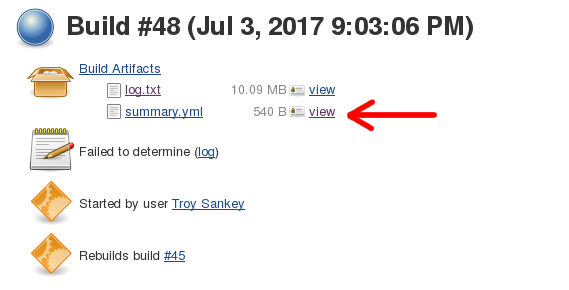
\includegraphics[height=12em]{summary_artifact.png}}
      \pause
\item NewRelic provides deeper application insight.\pause
% TODO: examples
\item Custom metrics in edx-platform: make use of the custom metrics middleware
      for peering into application behavior.
\end{itemize}
\end{frame}


\begin{frame}
\frametitle{Record Your Findings}
\begin{itemize}
\item Create a wiki page before testing.\pause
% This is a place where you should keep all data, scripts, configuration, and
% test results.  Armed with the wiki page, another person should be able to
% reproduce your test.
\item Caution: Beware of NewRelic data atrophie. NR gets hungry and eats your
      old dots.\pause
% Anything over 7 days old is of varying levels of quality.
\item Continuous deployment $\Rightarrow$ continuous deletion of system metrics!
% What instances?  They were terminated yesterday!
\end{itemize}
\end{frame}


\begin{frame}
\frametitle{Distributed load testing}
\begin{itemize}
\item Just run multiple load tests simultaneously in Jenkins.\pause
% * Locust distributed mode not currently implemented in run-simple-loadtest.
%   It would basically only award us the convenience of one click.
\item You may need to prime N workers first.\pause
\item If you want/need real distributed load testing, demand it!
% * Mention that the jenkins 2.0 upgrade is pseudo-blocking any further work on
%   run-simple-loadtest job enhancements.
\end{itemize}
\end{frame}


\begin{frame}
\frametitle{Maintaining load tests}
\begin{itemize}
\item Task ratios will rot.\pause
\item Tasks themselves will rot.\pause
\item New endpoints will need to be added as new tasks.
% If you never make sure they work, you may need to fix them every time you
% need them.  I'll be working on a notification system for indicating when a
% load test becomes obviously broken.
\end{itemize}
\end{frame}


\begin{frame}
\frametitle{For fun: Real browser load testing}
\begin{itemize}
\item \texttt{pip install realbrowserlocusts}, then subclass PhantomJSLocust in
      your locustfile.
\item Could make certain tests more realistic (AJAX calls actually happen).
% E.g. javascript changed to make more AJAX calls
\item Potentially far more resource intensive on the client side
% Javascript execution on the client likely becomes a bottleneck.
\end{itemize}
\end{frame}


\end{document}
